%!TEX root = report.tex
\subsection{Triangulation}
\label{sec:triangulation}

The basics for the triangulation technique are the camera projection equations \eqref{eq:projection}.
The difference is that in this case, one wants to find the real position of one point given its image points in images from multiple cameras. The governing equation is thus given by

\begin{align}
    \mathbf{x_j} & = C \quad P \quad \mathbf{X} \\
    s_j \begin{bmatrix} u_j \\ v_j \\ 1 \end{bmatrix} &= 
    C \begin{bmatrix} R \quad|\quad \mathbf{t} \end{bmatrix}
    \begin{bmatrix} X \\ Y \\  Z \\ 1 \end{bmatrix}, \quad \text{for }j=1\cdots N_{cameras}.
    \label{eq:triangulation}
 \end{align}

Both cases with fixed or free height $Z$ are considered. The resulting system of equations has 2 or 3 unknowns. 
The method applied is the one proposed by Hartley Zisserman (\cite{hz}, Chapter 12.2). 
First of all, for each camera, the following matrix needs to be set up. 

\begin{equation}
    \mathbf{A_j} = \begin{bmatrix} u_j \mathbf{f_3}-\mathbf{f_1} \\ v_j \mathbf{f_3}-\mathbf{f_2} \end{bmatrix},
\end{equation}

where $\mathbf{f_k}=P(k,:)$ denotes the $k$th row of the projection matrix and $u_j$,$v_j$ are the image points of the required point in Camera $j$.
The matrix $A$ is then composed of all rows $\mathbf{A_j}$, vertically stacked. It is of size $4\times(2 N_{cameras}$).

If the height is specified, then finding the solution to \eqref{eq:triangulation} comes back to solving

\begin{align}
    A'\mathbf{x}&=\mathbf{b}\\  
    \begin{bmatrix} \mathbf{a_1} & \mathbf{a_2} \end{bmatrix}^T \mathbf{x} &= -\mathbf{a_3}Z-\mathbf{a_4},
\end{align}

where $f_k$ denotes the $k$th row of the matrix $\mathbf{A}$
This system of equations can be solved in the least-squares sense, which leads to the solution $\mathbf{\hat{x}}=(A^TA)^{-1}A^T\mathbf{b}^T$. 
Adding the third component Z to $\mathbf{\hat{x}}$, the solution is obtained.

If the height is not specified, one can simply use a single value decomposition of $A$. The eigenvector with biggest eigenvalue corresponds to the solution of \eqref{eq:triangulation} in the least squares sense.

%\begin{lstlisting}[caption=Listing]
%\end{lstlisting}

%\begin{figure}[htb]
%	\centering
%	\begin{subfigure}[b]{0.49\linewidth}
%		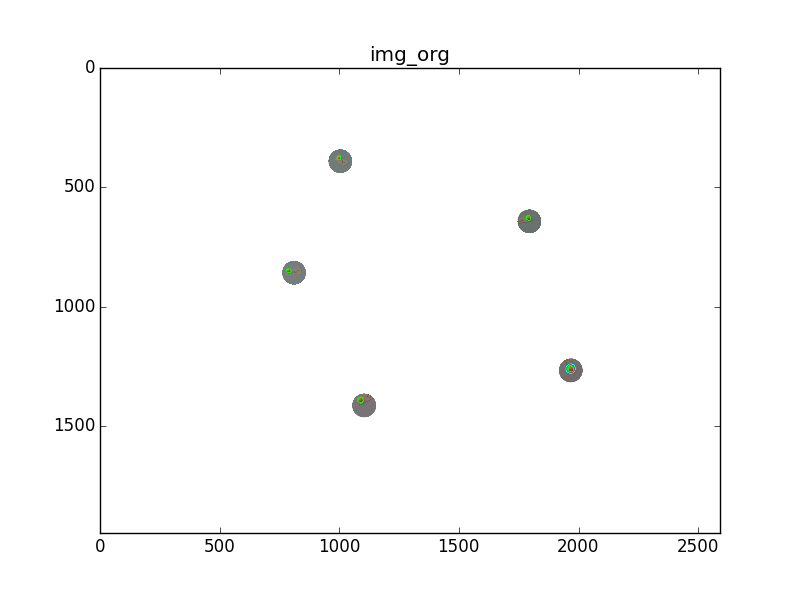
\includegraphics[width=\linewidth]{../files/img_org139.png}
%		\caption{Regions of interest chosen by user and extracted colors}
%		\label{feat_step0}
%	\end{subfigure}
%	\begin{subfigure}[b]{0.49\linewidth}
%		\includegraphics[width=\linewidth]{../files/img_h139.png}
%		\caption{\textit{Hue} representation of original image}
%		\label{feat_step1}
%	\end{subfigure}
%	\begin{subfigure}[b]{0.49\linewidth}
%		\includegraphics[width=\linewidth]{../files/img_s139.png}
%		\caption{\textit{Saturation} representation of original image}
%		\label{feat_step2}
%	\end{subfigure}
%	\begin{subfigure}[b]{0.49\linewidth}
%		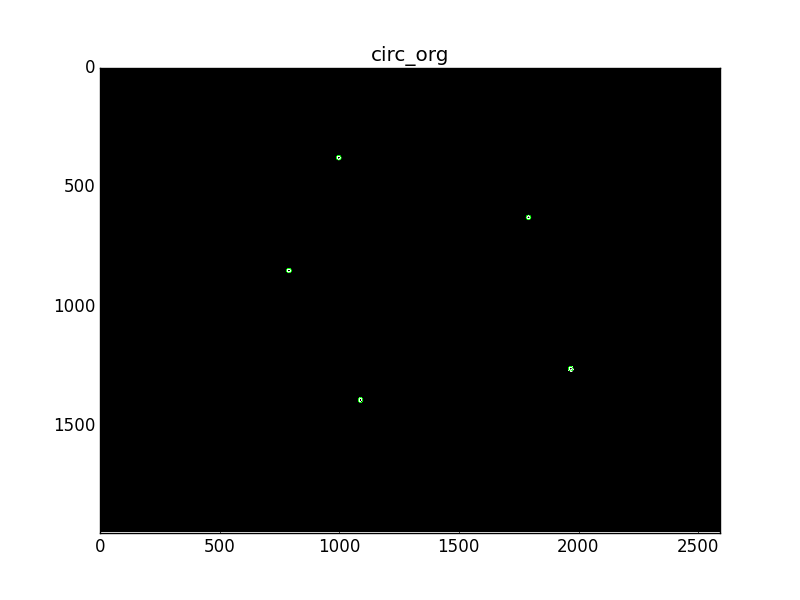
\includegraphics[width=\linewidth]{../files/circ_org139.png}
%		\caption{Regions of interest chosen by user and extracted colors}
%		\label{feat_step3}
%	\end{subfigure}
%	
%	
%	\begin{subfigure}[b]{0.49\linewidth}
%		\includegraphics[width=\linewidth]{../files/zdot_RefTrackNL.png}
%	\end{subfigure}
%	\begin{subfigure}[b]{0.49\linewidth}
%		\includegraphics[width=\linewidth]{../files/speeds_RefTrackNL.png}
%	\end{subfigure}
%	\begin{subfigure}[b]{0.49\linewidth}
%		\includegraphics[width=\linewidth]{../files/xyz_RefTrackNL.png}
%	\end{subfigure}
%	\caption{Procedure for feature extraction} 
%	\label{features}
%\end{figure}
